\documentclass[en]{../../../../../../eplexam}

\usepackage{../../../../../../eplunits}
\usepackage{bm}

\newcommand{\Base}[1]{\hat{\mathbf{e}}_{#1}}
\newcommand{\Vect}[1]{\vec{\mathbf{e}}_{#1}}
\newcommand{\en}{\mathcal{E}}

\hypertitle{Radiation and communication systems}{7}{ELEC}{2795}{2019}{Janvier}{All}
{Alice Borbath \and Martin Braquet \and Daniel Defrenne \and Olivier Leblanc \and Maxime Wattiaux}
{Christophe Craeye, Danielle Janvier, Jérome Louveaux, Claude Oestges and Luc Vandendorpe}

\section{(4,5 points)}

Frequency: $f=\SI{75}{GHz}$.

\begin{figure}[ht!]
    \centering
    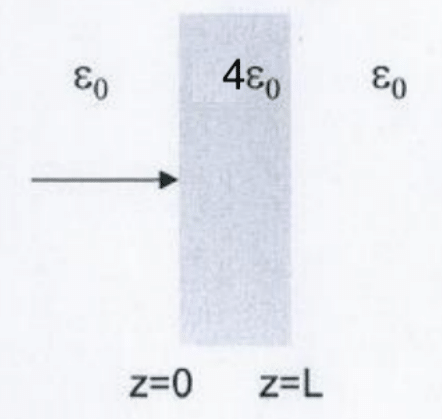
\includegraphics[scale=0.4]{Q1.png}
\end{figure}

\begin{enumerate}
    \item (1 point) Calculate the reflection coefficient at $z=0$.
    \item (1 point) Calculate the smallest value of $L$ such that there is total transmission at $z=0$ (in mm).
    \item (2,5 points) Assume that the frequency is not exactly at \SI{75}{GHz}, calculate the percentage of reflected power.
    Consider the frequency equal to $f=f_0(1+\delta)$ and develop to the first order of $\delta$.
    
    Hint: use $\sin(\pi+\epsilon)=-\sin(\epsilon)\approx-\epsilon$ and $\cos(\pi+\epsilon) \approx -1$ for $\epsilon \to 0$.
\end{enumerate}

\begin{solution}
 
\begin{enumerate}
 \item Let $Z_{eq}$ be the equivalent impedance at $z=0$ as seen by a wave propagating to the right:
 \[
  Z_{eq} = Z_c \frac{Z_L + j Z_c \tan(\beta L)}{Z_c + j Z_L \tan(\beta L)} = \frac{Z_0}{\sqrt{\epsilon_r}}\frac{Z_0 + j \frac{Z_0}{\sqrt{\epsilon_r}} \tan(\beta L)}{\frac{Z_0}{\sqrt{\epsilon_r}} + j Z_0 \tan(\beta L)} = \frac{Z_0}{\sqrt{\epsilon_r}}\frac{1 + j \frac{1}{\sqrt{\epsilon_r}} \tan(\beta L)}{\frac{1}{\sqrt{\epsilon_r}} + j \tan(\beta L)}
 \]
 where $\epsilon_r = 4$ is the relative permittivity in the central medium, $Z_L = Z_0$ is the impedance of the right medium, $Z_c = Z_0/\sqrt{\epsilon_r}$ is the characteristics impedance of the central medium, and $\beta = 2 \pi f \sqrt{\epsilon_r} / c$.
 
 The reflection coefficient is 
 \[
  \Gamma = \frac{Z_L - Z_c}{Z_L + Z_c} = \frac{j\left(\frac{1}{\epsilon_r} - 1 \right) \, \tan(\beta L)}{\frac{2}{\sqrt{\epsilon_r}} + j \left(\frac{1}{\epsilon_r} + 1\right) \tan(\beta L)} = \frac{j\left(\frac{1}{\epsilon_r} - 1 \right) \, \tan\left(\frac{2 \pi f}{c} \sqrt{\epsilon_r} L\right)}{\frac{2}{\sqrt{\epsilon_r}} + j \left(\frac{1}{\epsilon_r} + 1\right) \tan\left(\frac{2 \pi f}{c} \sqrt{\epsilon_r} L\right)}
 \]
 where $Z_L = Z_{eq}$ and $Z_c = Z_0$ is the characteristics impedance of the left medium.
 \item 
 \[
  \tan(\beta L) = 0 \quad \Leftrightarrow \quad \beta L = \pi \quad \Leftrightarrow \quad L = \frac{c}{2 \sqrt{\epsilon_r} f} = \SI{1}{mm}
 \]
 \item 
 \[
  \tan\left(\frac{2 \pi f_0 (1+\delta)}{c} \sqrt{\epsilon_r} L\right) = \tan\left(\pi + \underbrace{\frac{ 2 \pi f_0 \delta}{c} \sqrt{\epsilon_r} L}_{\epsilon}\right) \simeq \frac{-\left(\frac{ 2 \pi f_0 \delta}{c} \sqrt{\epsilon_r} L\right)}{-1} = \frac{ 2 \pi f_0 \delta}{c} \sqrt{\epsilon_r} L
 \]

 \[
  \Gamma = \frac{j\left(\frac{1}{\epsilon_r} - 1 \right) \, \frac{2 \pi f_0 \delta}{c} \sqrt{\epsilon_r} L}{\frac{2}{\sqrt{\epsilon_r}} + j \left(\frac{1}{\epsilon_r} + 1\right) \frac{2 \pi f_0 \delta}{c} \sqrt{\epsilon_r} L} = \frac{-2.36 \,  \delta j}{1+3.93 \,  \delta j}
 \]
 The percentage of reflected power is
 \[
  \abs{\Gamma}^2 = \frac{2.36^2 \, \delta^2}{1+3.93^2  \, \delta^2} = \frac{5.55 \, \delta^2}{1+15.4 \, \delta^2}.
 \]

\end{enumerate}
 
\end{solution}


\section{(4,5 points)}

A wireless horizontal link is established over a 100 meter distance at \SI{2.4}{GHz}. In first instance, we will assume that the antennas are placed high enough to be able to omit the effect of interaction with the ground. On the transmit side, the antenna is actually made of an array of two parallel half-wave dipoles, oriented perpendicularly to the ground and spaced by half a wavelength. The power fed to the pair of antennas is assumed to be split equally between the antennas, and the matching at the common feeding part is supposed perfect. On the receiving side, an antenna with circular polarization, with a 10 dB gain is used. The antenna is correctly pointed and its pattern falls off by 3 dB at an angle close to 25 degrees from boresight. That antenna is badly matched: it has an impedance of $100-20\imagj \Omega$, while the receiver has \SI{50}{\Omega} input impedance. Its noise figure is also relatively bad, corresponding to 4 dB. The transmitted array is not well pointed towards the receiving antenna, because of non-equal phases in the two excitations, such that the pattern is actually pointing 20 degrees away from the line of sight. The noise contributed by the environment will be calculated assuming a \SI{290}{K} temperature in all directions and the occupied bandwidth is \SI{20}{MHz}.

\begin{figure}[ht!]
    \centering
    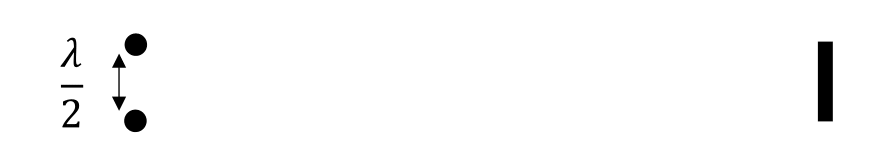
\includegraphics[scale=0.5]{Q2.png}
\end{figure}

\begin{enumerate}
    \item (4 points) Considering \SI{1}{mW} for the transmitting power, what is the SNR (in \si{dB}) observed at the receiver?
    \item (0,5 points) Please try to provide a rough estimate for an upper bound (in dB) of the (significant) effect of reflection on the ground, considering that the heights of the antennas above the ground are 20 meters.
\end{enumerate}

\begin{solution}

\begin{enumerate}
 \item The received power is 
 \[
  P_R = P_T \frac{L_R\,L_T\,G_R\,G_T}{L_{FS}}
 \]
 \begin{itemize}
  \item $ P_T = \SI{-30}{dB} $
  \item The impedance matching factor is 
  \[
   \abs{1-\Gamma}^2 = \abs{1-\frac{Z_L-Z_c}{Z_L+Z_c}}^2 = \abs{1-\frac{50 - 20 j}{150 - 20 j}}^2 = 0.437.
  \]
  The transmitter polarization is $ \Vect{i} = \frac{1}{\sqrt{2}} \left( 1 + \e^{j\pi\sin(\SI{20}{\degree}}\right) \Base{x} $ and the receiver polarization is $ \Base{p} = \frac{1}{\sqrt{2}} \left( \Base{x} + j \Base{y} \right)$. The polarization matching factor is
  \[
   \abs{\mathbf{\Vect{i}\cdot\Base{p}}}^2 = \abs{\frac{1}{\sqrt{2}} \left( 1 + \e^{j\pi\sin(\SI{20}{\degree}}\right)\frac{1}{\sqrt{2}}}^2 = 0.74.
  \]
  $ L_R = \abs{1-\Gamma}^2\abs{\mathbf{\Base{i}\cdot\Base{p}}}^2 = 0.323 = \SI{-4.89}{dB}$.
  \item $L_T = 1$.
  \item Since $\theta_{\SI{3}{dB}} = \frac{\SI{160}{\degree}}{\sqrt{G_R(u_0)}}$, $G_R(u_0) = \left(\frac{\SI{160}{\degree}}{25}\right)^2 = \SI{16.12}{dB}$. The gain of 10 dB has to be added: $G_R = \SI{26.12}{dB}$.
  \item $G_T = \SI{2.15}{dB}$ for a dipole.
  \item $L_{FS} = \SI{80.05}{dB}$.
 \end{itemize}

 The received power is thus
 \[
  P_R = -30 - 4.89 + 26.12 + 2.15 - 80.05 = \SI{-86.67}{dB}.
 \]
 The noise power is $N = kBT = \SI{-130.97}{dB}$.
 The output SNR is
 \[
  \mathrm{SNR}_o = \mathrm{SNR}_i / F = -86.67 + 130.97 -4 = \SI{40.3}{dB}.
 \]
 \item The angle of propagation for the reflected wave is $\theta = \arctan(20/50) = \SI{21.8}{\degree}$. It will create a wave being the sum of the waves from the two dipole. Taking into account the initial phase difference from the dipoles, the total phase shift is $ \pi (\sin(\SI{20}{\degree}) - \sin(\SI{21.8}{\degree}))$. The reflected wave is thus proportional to
 \[
  \gamma \left(1 + \e^{j \pi (\sin(\SI{20}{\degree}) - \sin(\SI{21.8}{\degree}))} \right)
 \]
 where $\gamma$ is the reflection coefficient, being equal to -1 for a small $\theta$.
 
 Depending on the position of the mobile receiver, the total amplitude will be the sum of the incident and reflected waves and will vary between
 \[
  \abs{1 + \e^{j \pi (\sin(\SI{20}{\degree}) - \sin(\SI{21.8}{\degree}))}} \pm \abs{1 + \e^{j \pi (\sin(\SI{20}{\degree}))}}
 \]
 The relative variation of the power is thus
 \[
  \left(\frac{\abs{1 + \e^{j \pi (\sin(\SI{20}{\degree}) - \sin(\SI{21.8}{\degree}))}} \pm \abs{1 + \e^{j \pi (\sin(\SI{20}{\degree}))}}}{\abs{1 + \e^{j \pi (\sin(\SI{20}{\degree}))}}}\right)^2,
 \]
 which corresponds to a variation ranging from -15.72 dB to 6.69 dB. The SNR is varying likewise.
\end{enumerate}


\end{solution}


\section{(4,5 points)}

Wireless transmission QPSK between 1 TX and 2 RX. The signal at antenna $i$ (1 or 2) is 
\[                                                                                    
    y_i(t)=h_i\sum_{n=0}^{N-1} I_nu(t-nT)+w_i(t)
\]
where 
\begin{itemize}
    \item $h_i$ is the fading coefficient between Rx and Tx;
    \item $I_n$ is the complex symbol sent at instant $nT$;
    \item $u(t)$ is the transmit filter;
    \item $w_i(t)$ is the complex envelope of the AWGN corrupting the signal, with bandpass power spectral density $\frac{N_i}{2}$. The noise between different Rx is uncorrelated.
\end{itemize}
We consider the detection operation to be performed by containing the two signals $y_1(t)$ and $y_2(t)$ to recover the transmitted data. We first apply a matched filter operation on signals $y_i(t)$ with a filter having impulse response $u^*(-t)$, and we sample the output at positions $mT$. This produces samples $y'_i[m]=h_iI_m\epsilon_u+w'_i[m]$ where $\epsilon_u$ is the energy contained in $u(t)$.
\begin{enumerate}
    \item Assuming first that $\frac{N_i}{2}=\frac{N_0}{2}$ for all $i$, (3 points)
    \begin{itemize}
        \item What is the decision rule corresponding to the ML estimate of $I_m$ based on both $y'_1[m]$ and $y'_2[m]$? Remark: don't forget $I_m$ is complex. Hint: find the ML estimate for the real part and the imaginary part.
        \item What can you say about the SNR of the decision variables? Comment please.
    \end{itemize}
    \item Let us consider that all $N_i$ can be different (1,5 points),
    \begin{itemize}
        \item Recalculate the ML decision rule for the data. 
        
        Hint: multiply each $y'[m]$ by a well-chosen term in order to obtain noise terms with equal variance.
        \item What can you say about the SNR of the decision variables compared to the SNR associated with each receive antenna? Comment please. What happens when for instance $N_1$ is much larger than $N_2$.
    \end{itemize}
\end{enumerate}

\begin{solution}

\begin{enumerate}
 \item 
 \begin{align*}
  \hat{I}_m &= \frac{\bm{h}^H \bm{y}}{\en_u \norm{\bm{h}}^2}\\
  P_N &= \frac{2 N_0}{\en_u \norm{\bm{h}}^2}\\
  P_S &= \sigma_I^2\\
  \mathrm{SNR} &= \frac{P_S}{P_N} = \frac{\en_s \norm{\bm{h}}^2}{N_0}
 \end{align*}
 The SNR is increased by the diversity (use of multiple receivers).
 \item 
 \begin{align*}
  \hat{I}_m &= \frac{\sum_{i=1}^2 h_i^* y_i / \sigma_{w_i'}^2}{\en_u \sum_{i=1}^2 \abs{h_i}^2 / \sigma_{w_i'}^2}\\
  P_N &= \frac{1}{\en_u^2 \sum_{i=1}^2 \abs{h_i}^2 / \sigma_{w_i'}^2} = \frac{1}{\en_u \sum_{i=1}^2 \abs{h_i}^2 / (2 N_i)}\\
  P_S &= \sigma_I^2\\
  \mathrm{SNR} &= \frac{P_S}{P_N} = \en_s \sum_{i=1}^2 \frac{\abs{h_i}^2}{N_i}
 \end{align*}
 The SNR increases when multiple receivers are used. If one antenna has a very large noise ($N_1 \gg N_2$), its associated term in the SNR drops to zero. This antenna is thus not used for the symbol prediction.
\end{enumerate}

\end{solution}


\section{(4,5 points)}

\begin{enumerate}
 \item 
If we consider a Ricean fading channel described
\begin{itemize}
    \item by a dominant multipath with a specific angle-of-arrival
    \item by a Rayleigh made of a large number of multipath arriving at the mobile terminal in the horizontal plane from all directions in azimuth.
\end{itemize}
In that case, the Doppler spectrum is given by:
\begin{enumerate}
    \item the so-called Jakes spectrum defined by 
    \[
     S(v) = \left\{ \begin{array}{ccc}
                  \frac{3}{2 \pi v_m \sqrt{1 - \frac{v^2}{v_m^2}}} & \textrm{for} &  \abs{v} < v_m \\
                  0 & \textrm{for} & \abs{v} \ge v_m
                  \end{array} \right.
    \]
    where $v_m$ is the maximum Doppler shift.
    \item a weighted combination of the Jakes spectrum and a delta function at the origin
    \item a weighted combination of the Jakes spectrum and a delta function centered at an adequate Doppler frequency
    \item a weighted combination of the so-called Jakes spectrum and a flat spectrum
\end{enumerate}

\item
In a hexadecimal cellular network characterized by a path-loss exponent equal to 3, a signal to interference ratio of 10 dB is targeted. The frequency reuse pattern must be based on at least 
    \begin{enumerate}
        \item 4 Cells
        \item 7 Cells
        \item 11 Cells
        \item 19 Cells
    \end{enumerate}

\item A cellular system operates in a Rayleigh fading channel such that the symbol period is smaller than the channel delay-spread. This implies that:
    \begin{enumerate}
        \item the channel creates inter-symbol interferences
        \item the channel transfer function is flat over the system bandwidth
        \item the coherence time of the channel cannot be defined
        \item the channel transfer function is real-valued
    \end{enumerate}

\item
Waveguiding propagation mechanisms (in corridors or street canyons) mostly cause
    \begin{enumerate}
        \item a large shadowing
        \item frequency selectivity
        \item a reduced Doppler frequency
        \item a path-loss exponent equal to 4
        \item a path-loss exponent lower than 2
    \end{enumerate}
    
\item
Suppose an electromagnetic wave coming from a transmitter with a circular polarization is propagating in a long street with high buildings. What is the best denomination for the polarization of the reflected wave? 

\begin{enumerate}
    \item circular
    \item elliptical
    \item horizontal linear
    \item vertical linear
    \item oriented linear 
\end{enumerate}

\item
In order to have the best VDSL system (best transmission), what can we say about cables? They must be:
    \begin{enumerate}
        \item no cables (wireless communication)
        \item shorter and thinner
        \item shorter and thicker
        \item longer and thinner
        \item longer and thicker
    \end{enumerate}
    
\item
What is the main advantage of OFDM that we can't find in DMT modulation?
    \begin{enumerate}
        \item Adapting the constellation size of each tone to SNR
        \item Allows easy implementation of FDD
        \item Taking benefit from frequency diversity
        \item \dots
        \item \dots
    \end{enumerate}
    
\item
What is the main purpose of twisted-pair wires?
\begin{enumerate}
    \item Reduce interferences for the differential mode
    \item Reduce interferences for the common mode
    \item Reduce the attenuation of the signal along its path
    \item Insert the wire more easily in the \dots
    \item Help for vectoring
\end{enumerate}

\item
Radio frequency interference (RFI):
\begin{enumerate}
    \item Signal with high power that affects all xDSL systems
    \item Signal with high power that \dots
    \item Signal with low power \dots
    \item Signal with low power \dots
    \item Signal with low power \dots
\end{enumerate}

\end{enumerate}

\begin{solution}
 \begin{enumerate}
  \item c. The Fourier transform of a complex exponential (auto-correlation function for a Ricean distribution) is a shifted delta.
  \item b. \[ K>\frac{1}{3} ((C/I) \, K_I)^{2/n} = 5.1 \]
  \item a
  \item e
  \item b
  \item c
  \item c
  \item a
  \item a
 \end{enumerate}

\end{solution}


\end{document}
